\documentclass[11pt,fleqn,oneside]{book} % Default font size and left-justified equations

\usepackage{fontawesome5}
\usepackage{booktabs}
\usepackage{tabularx}
\usepackage{graphicx}
\usepackage{biblatex}
\addbibresource{articles.bib}

\usepackage[autostyle=false, style=english]{csquotes}
\MakeOuterQuote{"}
% =======================================================================================
% Global settings
\newcommand{\AUTHOR}{Federico Brancasi}
\newcommand{\CLIENT}{Client Name}
\newcommand{\DATE}{\today}
\newcommand{\VERSION}{0.2.1}
\newcommand{\TITLE}{Blockchain}
\newcommand{\SUBTITLE}{University of Trento}
\newcommand{\SUBJECT}{UniTn}
\newcommand{\URL}{https://github.com/apehex}

%%%%%%%%%%%%%%%%%%%%%%%%%%%%%%%%%%%%%%%%%
% By Apehex
% github.com/apehex
%
% Built upon the The Legrand Orange Book by:
% Mathias Legrand (legrand.mathias@gmail.com)
%
% License:
% CC BY-NC-SA 3.0 (http://creativecommons.org/licenses/by-nc-sa/3.0/)
%
%%%%%%%%%%%%%%%%%%%%%%%%%%%%%%%%%%%%%%%%%

%------------------------------------------------------------------------------
%   GENERIC
%------------------------------------------------------------------------------

% ALL GENERIC FEATURES --------------------------------------------------------
%%%%%%%%%%%%%%%%%%%%%%%%%%%%%%%%%%%%%%%%%
% By Apehex
% github.com/apehex
%
% Built upon the The Legrand Orange Book by:
% Mathias Legrand (legrand.mathias@gmail.com)
%
% License:
% CC BY-NC-SA 3.0 (http://creativecommons.org/licenses/by-nc-sa/3.0/)
%
%%%%%%%%%%%%%%%%%%%%%%%%%%%%%%%%%%%%%%%%%

%------------------------------------------------------------------------------
%   GENERIC
%------------------------------------------------------------------------------

% THEMES ----------------------------------------------------------------------
%----------------------------------------------------------------------------------------
%   SOLVE CONFLICTS
%----------------------------------------------------------------------------------------
\PassOptionsToPackage{table}{xcolor}

%----------------------------------------------------------------------------------------
%   COLORS
%----------------------------------------------------------------------------------------
\usepackage[table]{xcolor} % Required for specifying colors by name
\usepackage{pagecolor} % dark theme
\definecolor{Orange}{HTML}{fa7303}
\definecolor{Blue}{HTML}{0e0441}
\definecolor{LightBlue}{HTML}{777294}
\definecolor{Snow}{HTML}{7fb1f7}
\definecolor{Hot}{HTML}{fe4003}
%----------------------------------------------------------------------------------------
%   MAKE BOLD STAND OUT
%----------------------------------------------------------------------------------------
\let\oldtextbf\textbf

%----------------------------------------------------------------------------------------
%   DARK THEME
%----------------------------------------------------------------------------------------
\newcommand{\togglethemedark}{
%----------------------------------------------------------------------------------------
\colorlet{accent}{orange}
\colorlet{fg}{white}
\colorlet{fgalt}{lightgray}
\colorlet{fgacc}{white}
\colorlet{bg}{black}
\colorlet{bgalt}{darkgray}
\colorlet{bgacc}{orange}
\colorlet{border}{white}
\colorlet{borderalt}{lightgray}
\colorlet{borderacc}{orange}
%----------------------------------------------------------------------------------------
\pagecolor{bg}
\color{fgalt}
\renewcommand{\textbf}[1]{\oldtextbf{\color{fg}##1}}
}

%----------------------------------------------------------------------------------------
%   LIGHT THEME
%----------------------------------------------------------------------------------------
\newcommand{\togglethemelight}{
%----------------------------------------------------------------------------------------
\colorlet{accent}{Orange}
\colorlet{fg}{black}
\colorlet{fgalt}{darkgray}
\colorlet{fgacc}{black}
\colorlet{bg}{white}
\colorlet{bgalt}{lightgray}
\colorlet{bgacc}{Blue}
\colorlet{border}{black}
\colorlet{borderalt}{darkgray}
\colorlet{borderacc}{orange}
%----------------------------------------------------------------------------------------
\pagecolor{bg}
\color{fgalt}
\renewcommand{\textbf}[1]{\oldtextbf{\color{fg}##1}}
}

%----------------------------------------------------------------------------------------
%   FORTA THEME
%----------------------------------------------------------------------------------------
\newcommand{\togglethemeforta}{
%----------------------------------------------------------------------------------------
\colorlet{accent}{white}
\colorlet{fg}{white}
\colorlet{fgalt}{lightgray}
\colorlet{fgacc}{black}
\colorlet{bg}{black}
\colorlet{bgalt}{darkgray}
\colorlet{bgacc}{white}
\colorlet{border}{white}
\colorlet{borderalt}{lightgray}
\colorlet{borderacc}{white}
%----------------------------------------------------------------------------------------
\pagecolor{bg}
\color{fgalt}
\renewcommand{\textbf}[1]{\oldtextbf{\color{fg}##1}}
}

\togglethemedark

% GEOMETRY --------------------------------------------------------------------
\usepackage{calc} % coordinate calculations

% PAGE LAYOUT -----------------------------------------------------------------
%----------------------------------------------------------------------------------------
%   PARAGRAPH FORMATING
%----------------------------------------------------------------------------------------

\setlength{\parindent}{0pt}
\setlength{\parskip}{12pt}

%----------------------------------------------------------------------------------------
%   FLOAT LAYOUT
%----------------------------------------------------------------------------------------

\renewcommand{\topfraction}{0.9}    % max fraction of floats at top
\renewcommand{\bottomfraction}{0.8} % max fraction of floats at bottom

%   Parameters for TEXT pages (not float pages):
\setcounter{topnumber}{2}
\setcounter{bottomnumber}{2}
\setcounter{totalnumber}{8}     % 2 may work better
\setcounter{dbltopnumber}{2}    % for 2-column pages
\renewcommand{\dbltopfraction}{0.9} % fit big float above 2-col. text
\renewcommand{\textfraction}{0.07}  % allow minimal text w. figs

%   Parameters for FLOAT pages (not text pages):
\renewcommand{\floatpagefraction}{0.7}  % require fuller float pages
\renewcommand{\dblfloatpagefraction}{0.7}   % require fuller float pages

% FONTS -----------------------------------------------------------------------
\usepackage{fontspec} % import new fonts
\usepackage[english]{babel}

%----------------------------------------------------------------------------------------
%   SPACING
%----------------------------------------------------------------------------------------

\usepackage{microtype}

%----------------------------------------------------------------------------------------
%   ADD BOLD + ITALIC
%----------------------------------------------------------------------------------------

\newfontfamily\inconsolatafontfamily[
    Path=template/generic/fonts/inconsolata/,
    Ligatures=TeX,
    Scale=MatchUppercase,
    UprightFont = *.otf,
    BoldFont = *-Bold.otf,
    ItalicFont = *-Italic.otf,
    BoldItalicFont = *-BoldItalic.otf
]{Inconsolata-LGC}

%----------------------------------------------------------------------------------------
%   FAMILY DEFAULTS
%----------------------------------------------------------------------------------------

% \setmonofont{\inconsolatafontfamily}
% \renewcommand*{\familydefault}{\ttdefault}

%----------------------------------------------------------------------------------------
%   HEADINGS
%----------------------------------------------------------------------------------------

\let\headingfontfamily\inconsolatafontfamily

% TITLES ----------------------------------------------------------------------
\usepackage{titlesec}

%----------------------------------------------------------------------------------------
%   SECTION NUMBERING IN THE MARGIN
%----------------------------------------------------------------------------------------

\newcommand{\autodot}{.} % separate title numbers with dots
\newcommand*{\numberinmargin}[3]{\makebox[0pt][r]{\textcolor{#3}{\fontsize{#2}{#2}\selectfont\headingfontfamily\bfseries\selectfont#1\autodot}\hskip\marginparsep}}

%----------------------------------------------------------------------------------------
%   LAYOUT
%----------------------------------------------------------------------------------------

\titlespacing*{\chapter}{0pt}{-30pt}{20pt}

\titlespacing*{\paragraph}{0pt}{3.25ex plus 1ex minus .2ex}{1.5ex plus .2ex}

%----------------------------------------------------------------------------------------
%   FORMAT
%----------------------------------------------------------------------------------------

\titleformat{\chapter}[hang]
  {\normalfont\huge\headingfontfamily\bfseries\selectfont\color{accent}}
  {\numberinmargin{\thechapter}{24}{accent}}
  {0pt}
  {\MakeUppercase}

\titleformat{\section}
  {\normalfont\large\headingfontfamily\bfseries\selectfont\color{fg}}
  {\numberinmargin{\thesection}{16}{accent}}
  {0pt}
  {\MakeUppercase}

\titleformat{\subsection}
  {\normalfont\normalsize\headingfontfamily\bfseries\selectfont\color{fg}}
  {\numberinmargin{\thesubsection}{12}{fg}}
  {0pt}
  {}

\titleformat{\subsubsection}
  {\normalfont\small\headingfontfamily\bfseries\selectfont\color{fg}}
  {\numberinmargin{\thesubsubsection}{10}{fg}}
  {0pt}
  {}

%----------------------------------------------------------------------------------------
%   SPECIAL TITLE
%----------------------------------------------------------------------------------------

\renewcommand{\paragraph}[1]{%
  \par\vspace{3.25ex plus 1ex minus .2ex}%
  \noindent\hspace*{-4cm}\colorbox{bgacc}{%
    \hspace*{4cm}\normalfont\huge\headingfontfamily\selectfont\color{fgacc}\uppercase{#1}
  }%
  \par\nobreak\vspace{1.5ex plus .2ex}%
}

% MATH ------------------------------------------------------------------------
\usepackage{amsmath,amsfonts,amssymb,amsthm} % For math equations, theorems, symbols, etc

% LINKS -----------------------------------------------------------------------
\usepackage{hyperref}
\usepackage{bookmark}
\usepackage[all]{hypcap} % moves the ref jumping points to the top of images (instead of the caption)

%----------------------------------------------------------------------------------------
%   HYPERLINKS IN THE DOCUMENTS
%----------------------------------------------------------------------------------------
\hypersetup{
hidelinks,
% backref=true,
% pagebackref=true,
% hyperindex=true,
colorlinks=true,
breaklinks=true,
urlcolor=accent,
% bookmarks=true,
bookmarksopen=false,
pdftitle={\TITLE},
pdfauthor={\AUTHOR},
pdfsubject={\SUBJECT}}

\bookmarksetup{
open,
numbered,
addtohook={%
\ifnum\bookmarkget{level}=0 % chapter
\bookmarksetup{bold}%
\fi
\ifnum\bookmarkget{level}=-1 % part
\bookmarksetup{color=accent,bold}%
\fi
}
}

%----------------------------------------------------------------------------------------
%   BOLD HREF
%----------------------------------------------------------------------------------------

\let\oldhref\href
\renewcommand{\href}[2]{\oldhref{#1}{\headingfontfamily\textbf{#2}}}

% LISTS -----------------------------------------------------------------------
\usepackage{enumitem} % Customize lists

%----------------------------------------------------------------------------------------
%   BULLET POINTS
%----------------------------------------------------------------------------------------

\setlist{nolistsep} % Reduce spacing between bullet points and numbered lists
\setlist[itemize]{leftmargin=4mm}
\setlist[enumerate]{leftmargin=4mm}

%----------------------------------------------------------------------------------------
%   DESCRIPTIONS
%----------------------------------------------------------------------------------------

% \newlength{\desclabelwidth}
% \setlength{\desclabelwidth}{4cm} % default value

% \renewenvironment{description}[1][4cm]
% {\setlength{\desclabelwidth}{#1}
% \begin{list}{}{
%     \renewcommand*{\makelabel}[1]{\bfseries##1\hspace{\desclabelwidth}}
%     \setlength{\itemsep}{0pt}
%     \setlength{\parsep}{0pt}
%     \setlength{\labelsep}{0pt}
%     \setlength{\leftmargin}{0pt}
%     \setlength{\itemindent}{\desclabelwidth}}}
% {\end{list}}

% CODE ------------------------------------------------------------------------
\usepackage{listings}

\input{template/generic/syntax/solidity}

% HEADERS ---------------------------------------------------------------------
\usepackage{fancyhdr} % Required for header and footer configuration

%----------------------------------------------------------------------------------------
%   PAGE HEADERS
%----------------------------------------------------------------------------------------

\fancypagestyle{plain}{%
    % Clear all headers and footers
    \fancyhf{}

    % Remove horizontal line in the header
    \renewcommand{\headrulewidth}{0pt}

    % Page number centered at the bottom
    \fancyfoot[C]{\thepage}
}

\fancypagestyle{fancy}{%
    % Clear all headers and footers
    \fancyhf{}

    % Remove horizontal line in the header
    \renewcommand{\headrulewidth}{0pt}

    % Page number centered at the bottom
    \fancyfoot[C]{\thepage}
}

% BOXES -----------------------------------------------------------------------
\usepackage[most]{tcolorbox}

%----------------------------------------------------------------------------------------
%   HIGHLIGHT ENVIRONMENT
%----------------------------------------------------------------------------------------

\newtcolorbox{highlight}{
  colback=bg,
  colframe=accent,
  coltext=fg,
  boxrule=2pt,
  boxsep=4pt,
  arc=0pt,
  outer arc=0pt
}

%----------------------------------------------------------------------------------------
%   REMARK ENVIRONMENT
%----------------------------------------------------------------------------------------

\newtcolorbox{remark}{
  colback=bg,
  colframe=accent,
  coltext=fg,
  boxrule=0pt,
  leftrule=2pt,
  boxsep=4pt,
  arc=0pt,
  outer arc=0pt,
}

\newtcolorbox{remark2}{
  colback=bg,
  colframe=Blue,
  coltext=fg,
  boxrule=0pt,
  leftrule=2pt,
  boxsep=4pt,
  arc=0pt,
  outer arc=0pt,
}

%----------------------------------------------------------------------------------------
%   OUTLINE ENVIRONMENT
%----------------------------------------------------------------------------------------

\newtcolorbox{outline}[1][4pt]{
  enhanced,
  colback=bg,
  colframe=bg, % To essentially hide the frame, but we will draw the corners manually
  coltext=fg,
  boxrule=0pt,
  boxsep=#1,
  arc=0pt,
  outer arc=0pt,
  overlay={
    % Top left corner
    \draw[Blue,line width=2pt] 
      (frame.north west) -- ++(0,-0.25*\tcbtextheight)
      (frame.north west) -- ++(0.25*\tcbtextwidth,0);
    % Bottom right corner
    \draw[Blue,line width=2pt]
      (frame.south east) -- ++(0,0.25*\tcbtextheight)
      (frame.south east) -- ++(-0.25*\tcbtextwidth,0);
  }
}

\newtcolorbox{outline2}[1][4pt]{
  enhanced,
  colback=bg,
  colframe=bg, % To essentially hide the frame, but we will draw the corners manually
  coltext=fg,
  boxrule=0pt,
  boxsep=#1,
  arc=0pt,
  outer arc=0pt,
  overlay={
    % Top left corner
    \draw[accent,line width=2pt] 
      (frame.north west) -- ++(0,-0.25*\tcbtextheight)
      (frame.north west) -- ++(0.25*\tcbtextwidth,0);
    % Bottom right corner
    \draw[accent,line width=2pt]
      (frame.south east) -- ++(0,0.25*\tcbtextheight)
      (frame.south east) -- ++(-0.25*\tcbtextwidth,0);
  }
}

% CAPTIONS --------------------------------------------------------------------
\usepackage{caption}

%----------------------------------------------------------------------------------------
%   COMMON
%----------------------------------------------------------------------------------------

\DeclareCaptionFont{fg}{\color{fg}}
\DeclareCaptionFont{accent}{\color{accent}}

%----------------------------------------------------------------------------------------
%   CODE: LSTLISTING
%----------------------------------------------------------------------------------------

\DeclareCaptionFormat{listing}{\colorbox{border}{\parbox{\dimexpr\linewidth-2\fboxsep\relax}{#1#2#3}}}
\captionsetup[lstlisting]{
  format=listing,
  labelfont=accent,
  textfont=fg,
  labelformat=empty,
  listformat=empty,
  singlelinecheck=false,
  margin=0pt,
  font={bf,footnotesize}
}

%----------------------------------------------------------------------------------------
%   TABLES
%----------------------------------------------------------------------------------------

\captionsetup[table]{
  labelformat=empty,
  listformat=empty,
}


%----------------------------------------------------------------------------------------
%   FIGURES
%----------------------------------------------------------------------------------------

\captionsetup[figure]{
  labelformat=empty,
  listformat=empty,
}

% ILLUSTRATIONS ---------------------------------------------------------------
\usepackage{graphicx} % Required for including pictures
\graphicspath{{images/}} % Specifies the directory where pictures are stored

\usepackage{tikz} % Required for drawing custom shapes
\usetikzlibrary{arrows, backgrounds, calc, fit, math, mindmap, positioning, shapes, shapes.geometric, tikzmark}

%----------------------------------------------------------------------------------------
%   GEOMETRY
%----------------------------------------------------------------------------------------

\newcommand{\drawhexagon}[5]{
    % #1 - text
    % #2 - position
    % #3 - size
    % #4 - rotation
    % #5 - options
    \node[rounded corners, inner sep=0, ultra thick, regular polygon, regular polygon sides=6, minimum size=#3, rotate=#4, #5] at (#2) {#1}
}

\newcommand{\drawtext}[5]{
    % #1 - text
    % #2 - position
    % #3 - height
    % #4 - rotation
    % #5 - options
    \node[left, bg, rounded corners, minimum width=\paperwidth, minimum height=#3, text width=\paperwidth, rotate=#4, #5] at (#2){#1}
}

\newcommand\pentagonvertex[5]{
    % #1 - Ox
    % #2 - Oy
    % #3 - R, radius of the outer circle including the vertexes
    % #4 - Theta, the tilt angle
    % #5 - I, index of the vertex
    ({#1 + #3*cos(72*#5 + #4)},%
     {#2 + #3*sin(72*#5 + #4)})%
}

%----------------------------------------------------------------------------------------
%   NODE TYPES
%----------------------------------------------------------------------------------------

\tikzstyle{title} = [
    minimum width=3cm,
    draw=none,
    text=fg,
    font=\bf,
    inner sep=0pt]

\tikzstyle{line} = [
    draw=border,
    -latex',
    very thick]

\tikzstyle{arrow} = [
    ->,
    >=stealth,
    draw=border,
    very thick]

\tikzstyle{label} = [
    text centered,
    text=fg,
    very thick]

\tikzstyle{startstop} = [
    rectangle,
    rounded corners,
    text centered,
    draw=border,
    fill=bg,
    text=fg,
    very thick,
    inner sep=2mm]

\tikzstyle{io} = [
    trapezium,
    trapezium left angle=70,
    trapezium right angle=110,
    text centered,
    draw=border,
    fill=bg,
    text=fg,
    very thick,
    inner sep=2mm]

\tikzstyle{container} = [
    rectangle,
    draw=border,
    dashed,
    very thick,
    text=fg,
    inner sep=4mm]

\tikzstyle{block} = [
    rectangle,
    text centered,
    draw=border,
    fill=bg,
    text=fg,
    very thick,
    inner sep=2mm]

\tikzstyle{decision} = [
    diamond,
    aspect=2,
    text centered,
    draw=border,
    fill=bg,
    text=fg,
    very thick,
    inner sep=2mm]

% TABLES ----------------------------------------------------------------------
\usepackage{booktabs} % Required for nicer horizontal rules in tables

%----------------------------------------------------------------------------------------
%   LINES
%----------------------------------------------------------------------------------------

% \arrayrulecolor{border}
% \setlength{\arrayrulewidth}{2pt} 

%----------------------------------------------------------------------------------------
%   LAYOUT
%----------------------------------------------------------------------------------------

% Define a new column type
\newcolumntype{C}{>{\color{fg}\large\centering\arraybackslash\hspace{16pt}}c<{\hspace{16pt}}}
\newcolumntype{L}{>{\color{fg}\large\raggedright\arraybackslash\hspace{16pt}}l<{\hspace{16pt}}}
\newcolumntype{R}{>{\color{fg}\large\raggedleft\arraybackslash\hspace{16pt}}r<{\hspace{16pt}}}

% Adjust the vertical padding
\renewcommand{\arraystretch}{1.5}

%----------------------------------------------------------------------------------------
%   HEADERS
%----------------------------------------------------------------------------------------

\newcommand{\thead}[1]{\large\uppercase{#1}}



%------------------------------------------------------------------------------
%   BOOK
%------------------------------------------------------------------------------

% PAGE LAYOUT -----------------------------------------------------------------
%----------------------------------------------------------------------------------------
%   GEOMETRY
%----------------------------------------------------------------------------------------

\usepackage[top=2cm,bottom=2cm,left=4cm,right=2cm,headsep=10pt,a4paper]{geometry} % margins

%----------------------------------------------------------------------------------------
%   LANDSCAPE
%----------------------------------------------------------------------------------------

\usepackage{pdflscape}

% TITLES ----------------------------------------------------------------------
\usepackage{titlesec}

%----------------------------------------------------------------------------------------
%   SET TEXT FOR THE PART PAGE
%----------------------------------------------------------------------------------------

\newcommand{\currentparttitle}{}
\newcommand{\currentpartintro}{}
\newcommand{\setparttitle}[1]{\renewcommand{\currentparttitle}{#1}}
\newcommand{\setpartintro}[1]{\renewcommand{\currentpartintro}{#1}}

%----------------------------------------------------------------------------------------
%   LAYOUT
%----------------------------------------------------------------------------------------

\titlespacing*{\part}{-3cm}{9cm}{20pt}

%----------------------------------------------------------------------------------------
%   FORMAT
%----------------------------------------------------------------------------------------

\titleformat{\part}[display]
  {}
  {}
  {0pt}
  {\begin{tikzpicture}[overlay]
    % horizontal bg strip behind title
    \node[anchor=north west, inner sep=0mm, outer sep=0pt, minimum height=48mm, minimum width=\paperwidth, xshift=0cm, yshift=2.8cm, fill=bg] {\parbox{\paperwidth}{}};
    % introduction block below title
    \node[anchor=north west, inner sep=0pt, outer sep=0pt, minimum height=48mm, minimum width=\paperwidth, xshift=0cm, yshift=-4cm, align=left] {\currentpartintro};
  \end{tikzpicture}
  \fontsize{48}{60}\headingfontfamily\color{fg}\MakeUppercase}

\let\originalpart\part

\renewcommand{\part}[1]{% to reference the title in the left bar in the margin
\setparttitle{\uppercase{#1}}
\backgroundtitlevisiblefalse
\originalpart{#1}
\backgroundtitlevisibletrue}

% COVER -----------------------------------------------------------------------
\newcommand{\coverpage}[5]{
    % #1 - title
    % #2 - subtitle
    % #3 - author
    % #4 - date
    % #5 - subject
    \pagestyle{empty}
    \newgeometry{left=0cm,top=0cm,right=0cm,bottom=0cm}

    \begin{tikzpicture}[remember picture,overlay]

    %%%%%%%%%%%%%%%%%%%% Layers %%%%%%%%%%%%%%%%%%%%%%%%
    \pgfdeclarelayer{bg}    % declare background layer
    \pgfdeclarelayer{fg}    % declare background layer
    \pgfsetlayers{bg,main,fg}  % set the order of the layers (main is the standard layer)

    %%%%%%%%%%%%%%%%%%%% Background %%%%%%%%%%%%%%%%%%%%%%%%
    \fill[bg] (current page.south west) rectangle (current page.north east);

    %%%%%%%%%%%%%%%%%%%% Background Polygon %%%%%%%%%%%%%%%%%%%%

    % top left
    \foreach \i in {0.5,...,20} {\drawhexagon{}{$(current page.north west)+(2.5,0)$}{\i cm}{0}{accent!60, draw=Orange};}

    % bottom left
    \foreach \i in {2.5,...,22} {\drawhexagon{}{$(current page.west)+(2.5,-5)$}{\i cm}{0}{accent!60,draw=Blue};}

    % center right
    \foreach \i in {0.5,...,22} {\drawhexagon{}{$(current page.north east)+(0,-9.5)$}{\i cm}{0}{accent!90,draw=Orange};}

    % bottom right
    \foreach \i in {21,...,2} {\drawhexagon{}{$(current page.south east)+(-0.2,-0.45)$}{\i cm}{0}{accent!85,draw=Blue};}

    %%%%%%%%%%%%%%%%%%%% Title + Subtitle %%%%%%%%%%%%%%%%%%%%
    \drawtext{\fontsize{48}{16}\textsc{\textbf{#1}}}{$(current page.center)+(3.7,-4)$}{3cm}{-60}{text=fg,align=right,font=\headingfontfamily};

    %%%%%%%%%%%%%%%%%%%% Author Name %%%%%%%%%%%%%%%%%%%%
    \begin{pgfonlayer}{fg}
    \drawtext{\Large\textsc{#3}\\\Large\textsc{#4}}{$(current page.east)+(-0.5,-5.2)$}{2cm}{0}{text=fg,anchor=east,align=right,font=\headingfontfamily};
    \end{pgfonlayer}

    %%%%%%%%%%%%%%%%%%%% Year %%%%%%%%%%%%%%%%%%%%
    \drawhexagon{\Large #5}{$(current page.west)+(2.5,-5)$}{2.5 cm}{0}{accent!60,draw,text=fg,font=\headingfontfamily, draw=Blue};

    \end{tikzpicture}
    \restoregeometry
}

% TOC -------------------------------------------------------------------------
\usepackage{titletoc} % Required for manipulating the table of contents
\usepackage{csquotes}
\usepackage{silence}
\WarningsOff[everypage]
\WarningsOff[caption]

\makeatletter

%----------------------------------------------------------------------------------------
%   PAGE LAYOUT
%----------------------------------------------------------------------------------------

\renewcommand{\tableofcontents}{
\backgroundbarvisiblefalse
\pagestyle{empty} % No headers
\newgeometry{left=0cm} % No left margin
\setcounter{tocdepth}{1} % TOC depth

{
\setlength{\parskip}{0pt}
\hypersetup{
hidelinks,
% backref=true,
% pagebackref=true,
% hyperindex=true,
% colorlinks=true,
breaklinks=true,
urlcolor=accent,
% bookmarks=true,
bookmarksopen=false,
pdftitle={\TITLE},
pdfauthor={\AUTHOR},
pdfsubject={\SUBJECT}
}
\@starttoc{toc}
}

\clearpage
\pagestyle{fancy} % Print headers again
\restoregeometry
\backgroundbarvisibletrue}

%----------------------------------------------------------------------------------------
%   LINE FORMATS
%----------------------------------------------------------------------------------------

% Part text styling
\renewcommand*\l@part[2]{%
\ifnum \c@tocdepth >-2
  \addpenalty{-\@highpenalty}%
  \vskip 0em
  \begingroup
    \parindent \z@ \rightskip \@pnumwidth
    \leavevmode\colorbox{Blue}{\vtop{\hsize=\dimexpr\textwidth\relax
      \strut\color{white}\bfseries\sffamily\uppercase{#1}%
      \nobreak\hfill\nobreak\hb@xt@\@pnumwidth{\hss #2}\strut}}\par
    \penalty\@highpenalty
  \endgroup
\fi}

% Chapter text styling
\renewcommand*\l@chapter[2]{%
\ifnum \c@tocdepth >\m@ne
  \addpenalty{-\@highpenalty}%
  \vskip 0pt
  \begingroup
    \parindent \z@ \rightskip \@pnumwidth
    \leavevmode\colorbox{Blue}{\vtop{\hsize=\dimexpr\textwidth\relax
      \hspace*{4cm}\strut\color{white}\bfseries\sffamily\uppercase{#1}
      \nobreak\hfill\nobreak\hb@xt@\@pnumwidth{\hss #2}\strut}}\par
    \penalty\@highpenalty
  \endgroup
\fi}

% Section text styling
\renewcommand*\l@section[2]{%
\ifnum \c@tocdepth >\z@
  \addpenalty{-\@highpenalty}%
  \vskip 0em
  \begingroup
    \parindent \z@ \rightskip \@pnumwidth
    \leavevmode\colorbox{bg}{\vtop{\hsize=\dimexpr\textwidth\relax
      \hspace*{4cm}\strut\color{fg}\sffamily#1
      \nobreak\hfill\nobreak\hb@xt@\@pnumwidth{\hss #2}\strut}}\par
    \penalty\@highpenalty
  \endgroup
\fi}

% Subsection text styling
\renewcommand*\l@subsection[2]{%
\ifnum \c@tocdepth >1
  \addpenalty{-\@highpenalty}%
  \vskip 0em
  \begingroup
    \parindent \z@ \rightskip \@pnumwidth
    \leavevmode\colorbox{bg}{\vtop{\hsize=\dimexpr\textwidth\relax
      \hspace*{4cm}\strut\color{fg}\sffamily#1
      \nobreak\hfill\nobreak\hb@xt@\@pnumwidth{\hss #2}\strut}}\par
    \penalty\@highpenalty
  \endgroup
\fi}

%----------------------------------------------------------------------------------------
%   LIST OF FIGURES
%----------------------------------------------------------------------------------------

\hypersetup{linkcolor=fg}

\renewcommand\listfigurename{\paragraph{List of Figures}}

\titlecontents{figure}[2em]
{}
{\contentslabel{3em}}
{\hspace*{-3em}}
{\titlerule*{\ }\contentspage}

\pretocmd{\listoffigures}{\begin{outline}[4em]}{}{}
\apptocmd{\listoffigures}{\end{outline}}{}{}

%----------------------------------------------------------------------------------------
%   LIST OF TABLES
%----------------------------------------------------------------------------------------

\renewcommand\listtablename{\paragraph{List of Tables}}

\titlecontents{table}[2em]
{}
{\contentslabel{3em}}
{\hspace*{-3em}}
{\titlerule*{\ }\contentspage}

\pretocmd{\listoftables}{\begin{outline}[4em]}{}{}
\apptocmd{\listoftables}{\end{outline}}{}{}


%----------------------------------------------------------------------------------------
%   MINI TABLE OF CONTENTS IN PART HEADS
%----------------------------------------------------------------------------------------

% % Chapter text styling
% \titlecontents{lchapter}[0em] % Indenting
% {\addvspace{15pt}\large\sffamily\bfseries} % Spacing and font options for chapters
% {\color{fgacc}\contentslabel[\Large\thecontentslabel]{1.25cm}\color{fgacc}} % Chapter number
% {}  
% {\color{fgacc}\normalsize\sffamily\bfseries\;\titlerule*[.5pc]{.}\;\thecontentspage} % Page number

% % Section text styling
% \titlecontents{lsection}[0em] % Indenting
% {\sffamily\small} % Spacing and font options for sections
% {\contentslabel[\thecontentslabel]{1.25cm}} % Section number
% {}
% {}

% % Subsection text styling
% \titlecontents{lsubsection}[.5em] % Indentation
% {\normalfont\footnotesize\sffamily} % Font settings
% {}
% {}
% {}

\makeatother

% BACKGROUND ------------------------------------------------------------------
\usepackage[all]{background}

%----------------------------------------------------------------------------------------
%   SHOW / HIDE PART TITLE IN THE LEFT BAR
%----------------------------------------------------------------------------------------

\newif\ifbackgroundtitlevisible
\backgroundtitlevisibletrue

\newif\ifbackgroundbarvisible
\backgroundbarvisibletrue

%----------------------------------------------------------------------------------------
%   CONFIGURE LEFT BAR
%----------------------------------------------------------------------------------------

\backgroundsetup{
  scale=1,
  color=bgacc,
  opacity=1,
  angle=0,
  position=current page.south west,
  vshift=0mm,
  hshift=16mm, % Adjust the distance from the left edge of the page
  contents={%
    \tikz{
      % \fill[bgacc] (0,0) rectangle (6mm,16mm); % bottom bar, 6mm wide, 16mm tall
      \ifbackgroundbarvisible
        \fill[bgacc] (0,\paperheight) rectangle (8mm,-\paperheight); % bar width 6mm
      \fi
      \ifbackgroundtitlevisible
        \node[rotate=90, fgacc, font=\huge\bfseries\headingfontfamily, anchor=west] at (4mm, 16mm) {\currentparttitle};
      \fi
    }
  }
}

% BIBLIOGRAPHY ----------------------------------------------------------------
% \usepackage[style=alphabetic,citestyle=numeric,sorting=nyt,sortcites=true,autopunct=true,autolang=other,hyperref=true,abbreviate=false,backref=true]{biblatex}

% \usepackage{makeidx} % Required to make an index
% \makeindex % Tells LaTeX to create the files required for indexing


 % Commands and style of the template

% =======================================================================================
\togglethemelight

\newcommand*{\img}[1]{%
    \raisebox{-.3\baselineskip}{%
        \includegraphics[
        height=\baselineskip,
        width=\baselineskip,
        keepaspectratio,
        ]{#1}%
    }%
}

\begin{document}

\hypersetup{citecolor=Orange}

% =======================================================================================
%\cleardoublepage % Forces the first chapter to start on an odd page so it's on the right

% =======================================================================================
%                                   PREAMBLE
% =======================================================================================
\coverpage{\TITLE}{\SUBTITLE}{\AUTHOR}{\DATE}{\SUBJECT}
%----------------------------------------------------------------------------------------
\newpage
\tableofcontents

% =======================================================================================
%                                   CHAPTERS
% =======================================================================================
\newpage
\chapter{What is a Blockchain?}
\section{Definition}

Blockchain is an innovative technology introduced by \textbf{Satoshi Nakamoto} in 2008 through his famous paper \href{https://bitcoin.org/bitcoin.pdf}{"Bitcoin: A Peer-to-Peer Electronic Cash System"} \cite{bitcoinSatoshi}. It is a revolutionary cryptography-based electronic payment system designed to overcome the limitations of traditional systems and promote decentralization.

\begin{remark}
Defined as "\textit{a Blockchain}," each block contains a cryptographic hash of the previous block, a timestamp and transaction data. This blockchain structure makes each block inextricably linked to the others, creating an immutable and transparent digital ledger.
\end{remark}

Blockchain's basic purpose is to act as a decentralized ledger, which means that transactions are recorded permanently and immutably without the need for a central authority. It also enables consensus to be maintained in a trust-free environment, allowing unknown and potentially untrusted participants to collaborate securely.

Trade Ledger is not that far back in the history of accounting evolution. Interestingly, the double-entry accounting system described in Luca Pacioli's book has origins dating back to the possible influence of the Muslim accounting practice implemented by the Venetians \cite{accountingBooks}. So yes, ledgers are not new at all!

Now that we understand the essence of blockchain technology and its historical roots, let us delve into the concepts of \textbf{Distributed Ledgers} and \textbf{Decentralized Ledgers}. Understanding these concepts is critical as they form the backbone of various blockchain implementations.

\section{Decentralized Ledgers}
A decentralized ledger is essentially a registry that is managed and updated by multiple parties without the need for a central authority. Imagine this ledger as a document shared among several participants, but instead of being controlled by a single entity, it is distributed over a peer-to-peer (P2P) network. In this network, each node has a copy of the ledger and can verify its transactions.

\textbf{\textcolor{Orange}{Strengths}}:
\begin{itemize}
\item \textbf{Enhanced Security}: Because there is no central point of control, decentralized ledgers are less vulnerable to cyber attacks.
\item \textbf{Transparency and Accountability}: All parties involved can see and verify transactions, promoting transparency and accountability.
\item \textbf{Trustless Environments}: No need to rely on intermediaries to verify transactions, creating a trustless environment.
\end{itemize}

\vspace{2cm}

\textbf{\textcolor{Orange}{Drawbacks}}:
\begin{itemize}
\item \textbf{Processing Speed}: Due to the consensus required by multiple parties, transactions can be slower than in centralized systems.
\item \textbf{Complexity of Implementation}: Multi-party coordination and agreement are required to effectively implement a decentralized ledger.
\item \textbf{High Costs}: Maintaining the network requires significant resources in terms of computing power and energy.
\end{itemize}

\section{Distributed Ledgers}

A distributed ledger is a ledger that is managed and updated by multiple parties and stored in multiple locations. Unlike a decentralized ledger, which is distributed over a peer-to-peer network, a distributed ledger operates over a distributed network, where each node in the network owns a copy of the ledger and can validate transactions.

\textbf{\textcolor{Orange}{Strengths}}:

\begin{itemize}
    \item \textbf{Enhanced Processing Speed}: Distributed ledgers can be faster than decentralized ledgers because they can process transactions in parallel.
    \item \textbf{Improved Scalability}: Being more scalable than decentralized ledgers, distributed ledgers can be expanded to accommodate more users and transactions.
    \item \textbf{Increased Flexibility}: Distributed ledgers can be more flexible than decentralized ledgers because they can be customized to meet specific needs.
\end{itemize}

\textbf{\textcolor{Orange}{Drawbacks}}:

\begin{itemize}
    \item \textbf{Potentially Lower Security}: Unlike decentralized ledgers, distributed ledgers may be less secure because there is a central control point that could be targeted by hackers.
    \item \textbf{Reduced Transparency and Accountability}: Some parts of the network may have more control over the ledger than others, reducing overall transparency and accountability.
    \item \textbf{Complexity and Management}: Distributed ledgers can be more complex and difficult to manage than decentralized ledgers because they require coordination and agreement among multiple parties and multiple copies of the ledger.
\end{itemize}


\section{The Role of Trust and the Evolution of the Blockchain}

Trust plays a central role in understanding blockchain, going beyond mere technology and raising crucial philosophical and political questions concerning governance and the distribution of power.

Throughout history, philosophers and political theorists have examined different forms of social organization and the role of trust in institutions. From Plato to Hayek, perspectives vary widely, influencing our conceptions of power and trust.

The 2008 financial crisis acted as a catalyst for the adoption and development of blockchain and Bitcoin. The collapse of banks and financial institutions profoundly undermined trust in central institutions, pushing for greater decentralization and financial autonomy.

Moreover, blockchain does not simply represent a new technological invention, but rather an amalgamation of existing technologies that have been developed and refined over time. It is through the evolution of these technologies that blockchain has taken shape and begun to play a significant role in the digital landscape. To better understand this process, let us examine a rough timeline of key inventions:

\begin{figure}[htbp]
\centering
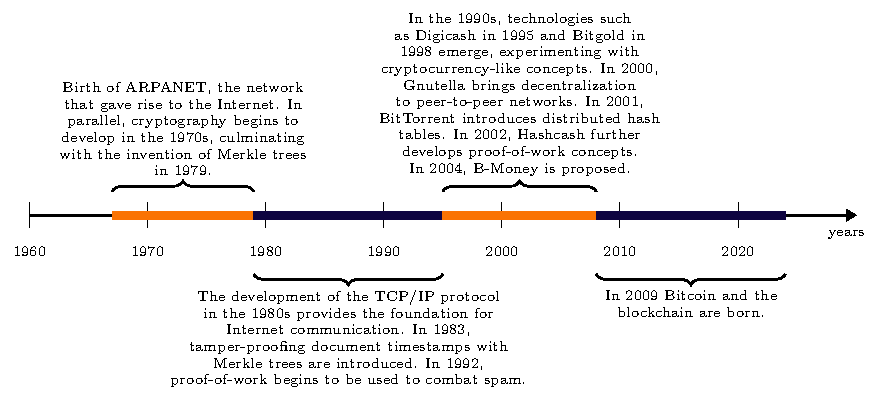
\includegraphics[width=1\textwidth]{tikz/chapter1 - Blockchain Timeline.pdf}
\caption{Blockchain Key Inventions Timeline}
\end{figure}

\newpage
\chapter{Blockchain Core Concepts}
\section{Decentralization/Distribution: What Sets Them Apart?}

Let us now restate the difference of the concepts of decentralization and distribution in the context of blockchain.

\begin{outline}
\textbf{Decentralization} refers to the distribution of control and decision-making power from a central authority. In blockchain, this means that no single entity has control over the network. Instead, the network is managed by a group of nodes that work together to maintain the integrity of the network.

\textbf{Distribution}, on the other hand, refers to the physical dispersion of data or computing resources in a network. In blockchain, this means that the data and computing resources needed to maintain the network are distributed across multiple nodes. This distribution makes blockchain technology extremely resilient and secure: even if one or more nodes go offline, the network can continue to function because the other nodes can assume their responsibilities.
\end{outline}


\section{Methods of Decentralization}
In this section, we will explore the three distinct degrees of decentralization and how they vary based on the implementation of two key concepts: \textbf{disintermediation} and \textbf{competition-driven decentralization}. 

\begin{enumerate}
\item \textbf{\textcolor{Blue}{Fully Centralized}}: In this case, all operations, controls and decisions are managed by a single central authority or entity. There is no form of decentralization. Disintermediation is absent and there is no competition for control of the network.

\item \textbf{\textcolor{Blue}{Semi-Decentralized}}: In a semi-decentralized structure, some aspects of the system are decentralized, while others are still centrally controlled. This may result in some degree of disintermediation, where some functions can be performed without third-party intervention, but is not completely eliminated. Competition-driven decentralization may be present in some parts of the system, but may not be applied in all aspects.

\item \textbf{\textcolor{Blue}{Fully Decentralized}}: In a fully decentralized system, there is no central authority controlling the system or making decisions. All operations are handled by network users in a distributed manner. This level of decentralization leads to strong disintermediation, where transactions and operations can take place directly between parties without intermediaries. In addition, competition for control of the network can be a key element, where network actors openly compete to influence consensus decisions.
\end{enumerate}

It is clear from the above explanations that decentralization and distribution are two crucial concepts in the design of blockchain networks. However, it is worth noting the \textit{subtle difference} between the two.

Decentralization deals with decision making and who has the power to make decisions (\textbf{governance}), while distribution deals with the physical arrangement of resources in the network (\textbf{technical concept}).

Interestingly, a network can be decentralized without being distributed, and vice versa. However, in practice, most decentralized networks are also distributed (this is because distribution is crucial to ensure network integrity and resilience).

\section{Unveiling the Core of Blockchain}
Finally, we reach the \textit{juiciest part}: the fundamental concepts of blockchain. Let's explore the pillars on which this revolutionary technology is based!

\textbf{\textcolor{Orange}{Nodes}}: Nodes constitute the cornerstone elements of the Blockchain community. They represent the participants or entities that drive the network. These can be computers, laptops or servers belonging to individuals or organizations. Each node assumes a crucial role in the blockchain architecture, contributing its resources and capabilities to the functioning of the entire system.

\textbf{\textcolor{Orange}{Transactions}}: Each transaction in the blockchain represents a major event permanently recorded in digital history. When two or more nodes interact, a transaction is noted in the blockchain through a process known as hashing. This process ensures the security and immutability of each transaction, preserving the integrity of the data transmitted.

\textbf{\textcolor{Orange}{Blockchain}}: Let us now imagine all these transactions organized and collected into blocks. Each block constitutes a key point in the blockchain's history, containing a series of related transactions. These blocks are linked consistently through consensus mechanisms, forming an unbroken chain of information.

\textbf{\textcolor{Orange}{Ledger}}: Finally, there is the ledger, the core of the blockchain. This distributed public ledger is hosted on all community nodes, representing the cornerstone of transparency and authenticity. Every block of transactions finds its place within this ledger, recorded sequentially and accessible to all participants. It is the trusted guardian of every movement and transaction within the blockchain.

\begin{figure}[hb]
\centering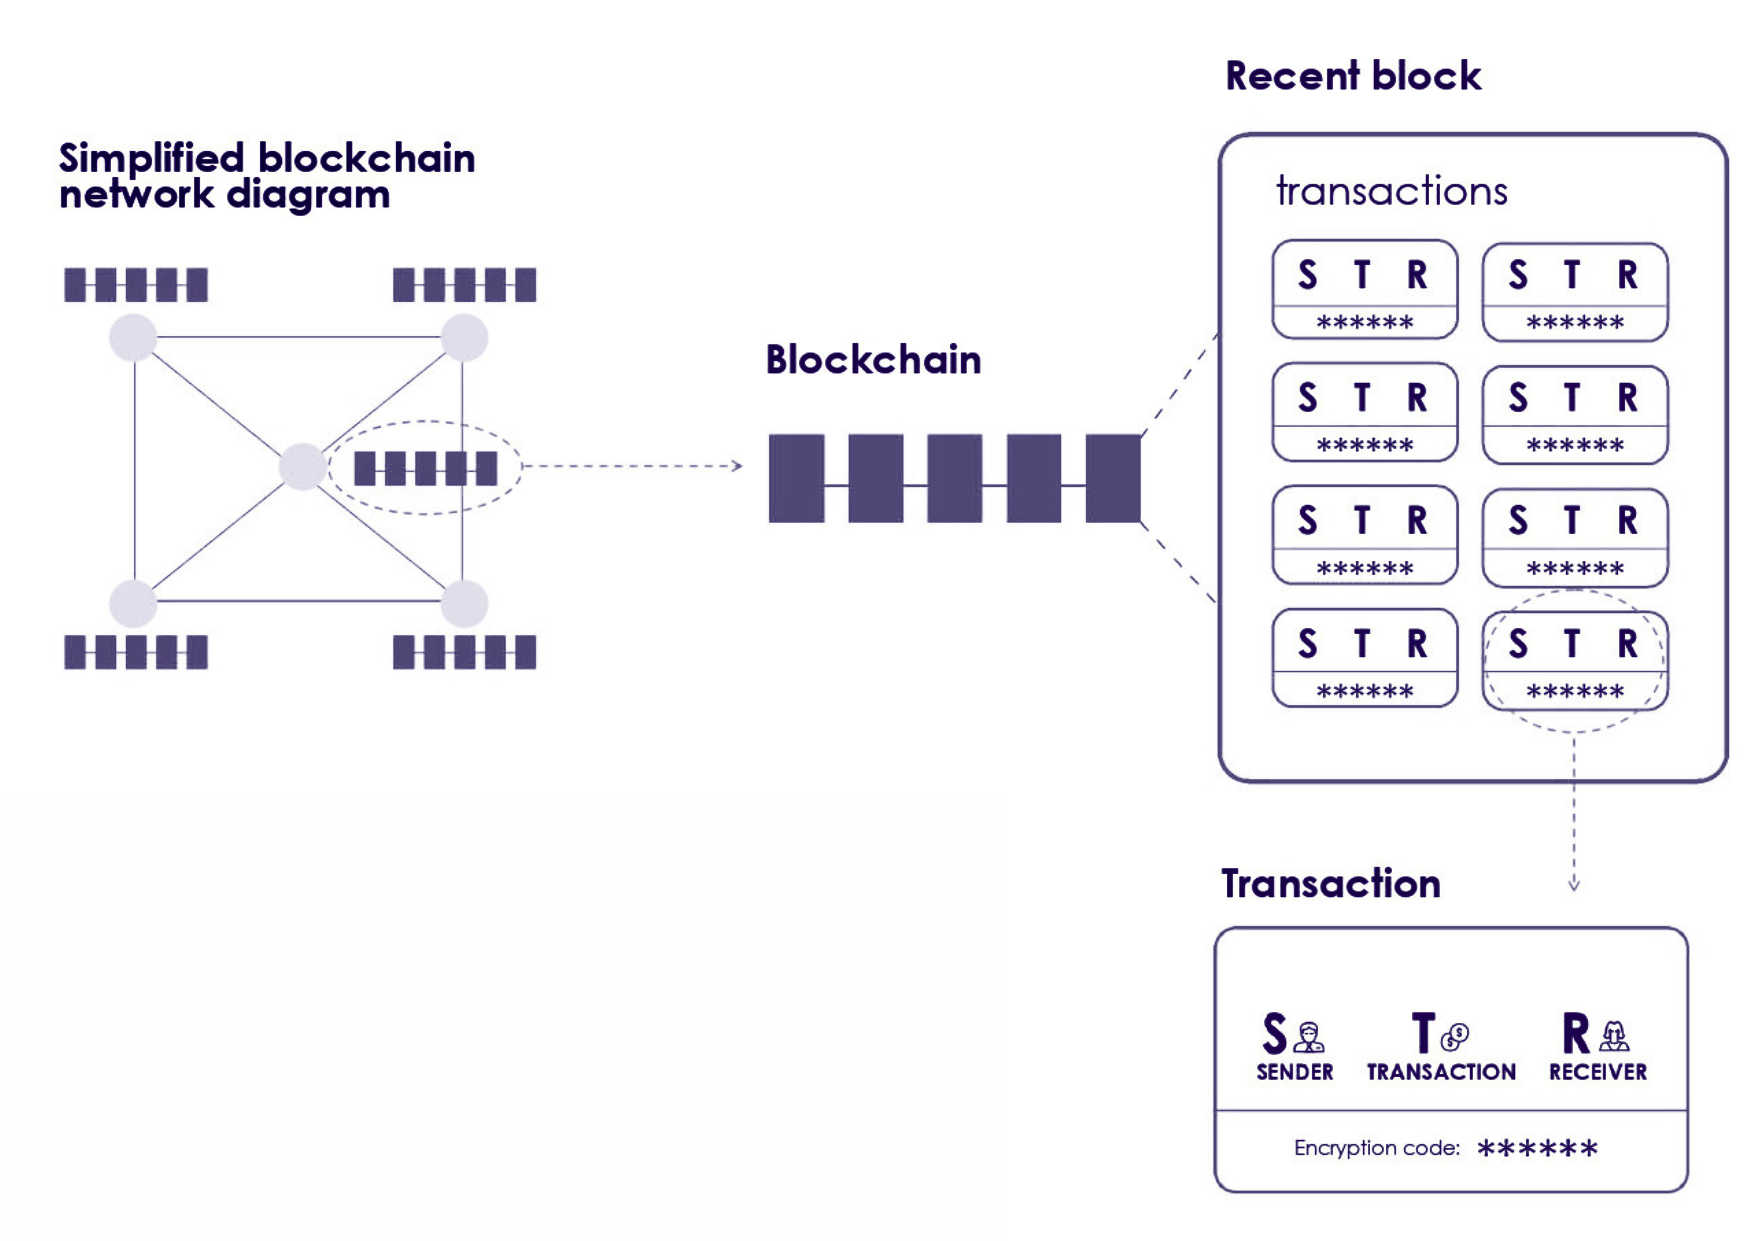
\includegraphics[scale=0.3]{tikz/chapter2 - Blockchain.png}
\caption{{\color{red}\colorbox{pink}{Tikz TODO}} Visual Example of the Blockchain \cite{blockchainFinyear}}
\end{figure}


\section{The Anatomy of a Block}

Let's go a little deeper! Let us now examine a block with a magnifying lens  \faSearch

\textbf{\textcolor{Blue}{Header}}:
\begin{itemize}
    \item \textbf{Hash of the Previous Header Link}: This field contains the hash value of the previous block, thus creating an immutable chain of blocks. Hashes, such as the popular SHA-256 (256-bit Secure Hash Algorithm), are cryptographic functions that transform data into fixed-length strings, which are essential for verifying data integrity.
    \item \textbf{Nonce}: This is an arbitrary value that is changed during the mining process until a hash is found that meets specific criteria.
    \item \textbf{Timestamp}: This indicates the precise time when the block was created.
    \item \textbf{Merkle Root}: This is the root hash of a Merkle tree, a data structure that enables efficient verification of the integrity of transactions contained in the block.
\end{itemize}


\textbf{\textcolor{Blue}{Body}}:
\begin{itemize}
    \item \textbf{List of Transactions}: This section lists all the transactions included in the block. Each transaction represents an exchange of value or data within the blockchain network, contributing to the traceability and security of transactions.
\end{itemize}

% \vspace{1cm}
\begin{figure}[hb]
\centering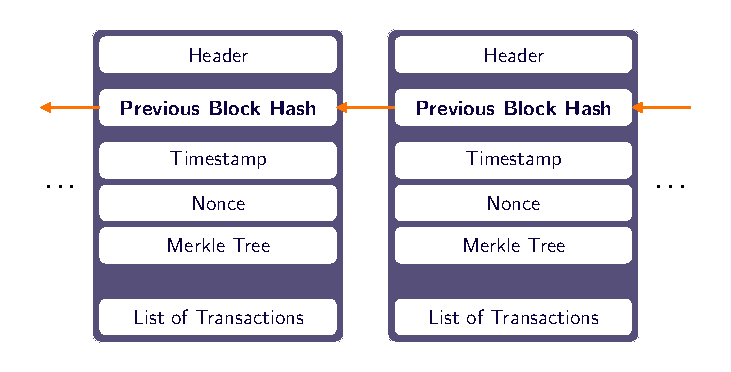
\includegraphics[scale=1.2]{tikz/chapter2 - Blocks.pdf}
\caption{Visual Example of the Blocks}
\end{figure}


\newpage
\chapter{Consensus Mechanisms}
\section{High Level Considerations}

Before diving into the details of consensus mechanisms, let's take a look at the advantages and limitations of using blockchain:

\begin{table}[h]
\begin{tabularx}{\linewidth}{>{\parskip1ex}X@{\kern4\tabcolsep}>{\parskip1ex}X}
\toprule
\hfil\bfseries \color{Orange}{Pros}
&
\hfil\bfseries \color{Orange}{Cons}
\\\cmidrule(r{3\tabcolsep}){1-1}\cmidrule(l{-\tabcolsep}){2-2}

%% PROS
Among the main benefits, \textbf{\color{Blue}{decentralization}} emerges as one of the key pillars, enabling a distributed network in which no central authority has absolute control. This not only increases the security and reliability of the network, but also promotes \textbf{\color{Blue}{transparency and trust}} among participants, making every transaction traceable and verifiable by anyone. In addition, the \textbf{\color{Blue}{immutability}} of data recorded on the blockchain, coupled with its \textbf{\color{Blue}{high availability}}, ensures that information is protected from manipulation and \textbf{\color{Blue}{always accessible}} when needed. These benefits, along with process simplification, efficiency in regulations and \textbf{\color{Blue}{cost savings}}, turn blockchain into a \textbf{\color{Blue}{reliable and programmable platform}} for a wide range of applications. Specifically, cost savings result from the elimination of intermediaries in transactions, enabling a direct transfer of value between the parties involved.
&

%% CONS
However, despite its advantages, blockchain technology also has some significant limitations that hinder its wider adoption. The appearance of the \textbf{\color{Blue}{new technology}}, for example, poses challenges in terms of familiarization and implementation for many organizations. In addition, the \textbf{\color{Blue}{scalability}} of blockchain, especially in public networks, may be limited with respect to the needs of high-frequency transactions. The issue of data \textbf{\color{Blue}{privacy and confidentiality}} remains an area of concern, as information recorded on the blockchain is permanent and accessible to all participants. \textbf{\color{Blue}{Limited adoption}}, \textbf{\color{Blue}{interoperability}} between different blockchain platforms, and complex \textbf{\color{Blue}{regulatory issues}} represent additional challenges that must be overcome to maximize the potential of blockchain technology.
\\\bottomrule
\end{tabularx}
\caption{Benefits and Limitations of Blockchain Technology}
\end{table}

\section{DLT Categories}
\textbf{Distributed Ledger Technologies} (DLTs) can be categorized in different ways based on their use and structure. One of the main categories is Blockchain, which is a specific type of DLT used for shared and immutable ledgers.

Blockchain can be further divided into three main types: public, private and consortium. \textbf{\textcolor{Blue}{Public blockchains}} are open to anyone who wants to participate and are decentralized. \textbf{\textcolor{Blue}{Private blockchains}} are controlled by a centralized organization or entity and are accessible only to authorized users. \textbf{\textcolor{Blue}{Consortial blockchains}} are managed by a group of organizations working together to manage the network.

In addition to blockchains, there are other types of DLTs such as Sidechains and Distributed Ledgers. \textbf{\textcolor{Blue}{Sidechains}} are blockchains linked to a main blockchain and can be used for specific purposes or to enhance the functionality (scalability) of the main blockchain. \textbf{\textcolor{Blue}{Distributed Ledgers}}, on the other hand, are shared ledgers that can be customized for specific purposes and are not necessarily blockchain-based.

\begin{figure}[h]
\centering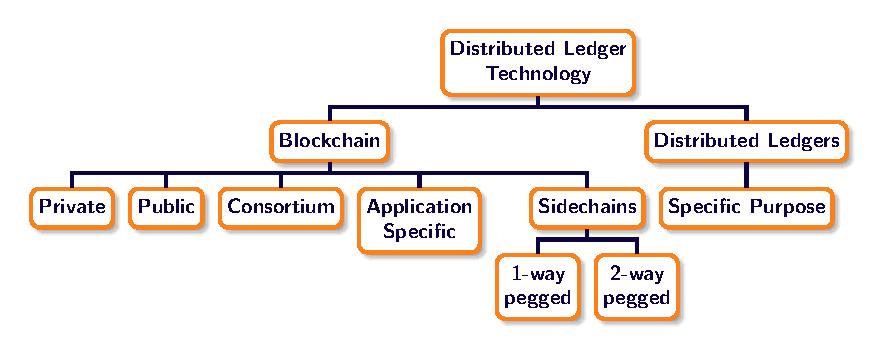
\includegraphics[scale=1]{tikz/chapter3 - DLT.pdf}
\caption{Distributed Ledger Technologies Categories}
\end{figure}

\section{Byzantine Generals Problems}
The Byzantine Generals problem is a fundamental concept in the context of distributed consensus mechanisms. Imagine a situation in which several commanders of an army must coordinate to attack or retreat, but some of them may be traitors or communications between them may be compromised. In this scenario, it is essential that the generals reach a consensus on the strategy to be adopted despite the uncertainty and the presence of potential mistakes or sabotage.

PBFT (Practical Byzantine Fault Tolerance) solves this problem by establishing a set of requirements to ensure reliable consensus among participants (Of course, we are no longer talking about battles, but about blockchain!). These requirements include:
\begin{itemize}
    \item \textbf{Agreement}: All nodes must agree on a single value proposition or decision.
    \item \textbf{Integrity}: Information and transactions must be authentic and unchanged during the consensus process.
    \item \textbf{Validity}: Only valid and legitimate transactions must be accepted and confirmed.
    \item \textbf{Fault Tolerance}: The system must be able to function properly even if some nodes fail or misbehave.
    \item \textbf{Termination}: The consensus process must eventually reach a conclusion and produce a final outcome.
\end{itemize}
Using PBFT, participants can collaborate safely and reliably even in the presence of faulty or malicious nodes. This consensus mechanism is critical to ensuring the consistency and reliability of transactions within distributed networks, such as those based on blockchain technology.

\vspace{2cm}
\section{Security Mechanisms}
In the blockchain, the application of security mechanisms is critical to ensure the security and integrity of transactions. These functions are used in different contexts, below we make a list and it is likely that you already know how some of them work.

\begin{remark}
\textbf{Cryptographic Hash Functions}:
Hash functions are fundamental in the blockchain and are used to confirm and validate new blocks of transactions, to create unique addresses for accounts on the blockchain, to verify the authenticity of messages sent over the network and in Merkle trees.
\end{remark}

\begin{remark2}
\textbf{Asymmetric cryptography}:
A cryptographic technique involving two keys: public and private. 
In the encryption process, the sender encrypts the message with the recipient's public key and, in the case of digital signatures, signs the message with his own private key, while the recipient verifies the signature using the sender's public key.
\end{remark2}

\begin{remark}
\textbf{Merkle trees}:
A data structure that ensures the integrity of transactions in the blockchain.
Transactions are organized in a binary tree, and hashes are used to ensure the integrity of the structure.
They allow for quick verification of whether a transaction is included in a blockchain without having to examine all transactions.
\end{remark}


\section{Type of Consensus Mechanisms}
When it comes to exploring the vast world of consensus mechanisms within blockchains, we are faced with a myriad of options. However, we will focus mainly on three of them: the Proof of Work, the Proof of Stake and the Delegated Proof of Stake. 

\faBitcoin \quad \textbf{Proof of Work} (PoW):

In PoW, participants, called "miners," compete to solve complex cryptographic puzzles.
The first miner to solve the puzzle gains the right to create and confirm a new block of transactions on the blockchain.
This process requires an enormous amount of computing power, making the system secure but also energy intensive.

\faEthereum \quad \textbf{Proof of Stake} (PoS):

In PoS, the right to create and validate a new block depends on the amount of cryptocurrency owned and "played" by participants, called "validators."
The more cryptocurrency that is "played," the greater the probability of being chosen to validate a block and receive rewards.
Because it does not require as intensive computing power as PoW, PoS is more energy efficient.

\faUsers \quad \textbf{Delegated Proof of Stake} (DPoS):

In DPoS, participants elect "delegates" responsible for creating and confirming blocks.
These delegates are voted on by other participants based on trust and reputation.
DPoS is designed to scale more efficiently than PoW and PoS, allowing for faster confirmation of transactions. 

\section{Blockchain Trilemma}


The trilemma of \textbf{decentralization}, \textbf{scalability} and \textbf{security} is one of the most significant challenges in designing and implementing an effective blockchain. The consensus mechanism plays a crucial role in balancing these three dimensions.

\begin{figure}[!htbp]
\centering
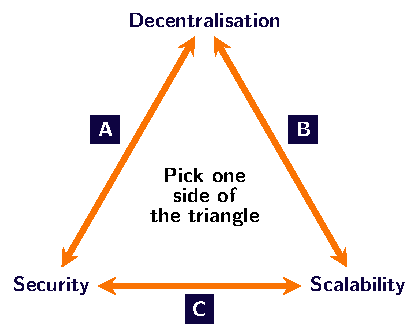
\includegraphics[width=0.6\linewidth]{tikz/chapter3 - Trilemma.pdf}
\caption{The Blockchain Trilemma}
\end{figure}

\textbf{\textcolor{Orange}{Decentralisation}} refers to the \textbf{distribution of decision-making power} among network participants rather than concentrating it in a single centralized entity. An effective consensus mechanism should ensure that no single actor or group of actors has complete control over the network, thus promoting decentralization. However, decentralization can be challenged by the need to reach agreement on transactions and state updates among geographically distributed nodes.

\textbf{\textcolor{Orange}{Scalability}} refers to the \textbf{ability of the system to handle an increasing number of transactions} and to grow efficiently as the workload increases. An efficient consensus mechanism should enable the network to process a large number of transactions quickly and economically without compromising its security or decentralization. However, achieving scalability can be hampered by the computational complexity and communication required to achieve distributed consensus.

\textbf{\textcolor{Orange}{Security} is critical} to \textbf{protect the network from malicious attacks, manipulation, and fraud}. A robust consensus mechanism should ensure the integrity and immutability of data stored on the blockchain, as well as resistance to attack attempts by malicious actors. However, maintaining a high level of security may require compromises on the speed or scalability of the network.

To address the trilemma, there are two main approaches in designing consensus mechanisms:
\begin{itemize}
    \item \textbf{Message-based consensus mechanisms}: in this approach, network participants communicate with each other to reach consensus on the validity of transactions and the state of the blockchain. 
    \item \textbf{Shared memory-based consensus mechanisms}: in this approach, participants share a common memory space and use synchronization techniques to ensure that all nodes in the network agree on the state of the system. 
\end{itemize}

\section{Distributed Consensus}
In the context of distributed systems, reaching consensus among nodes that do not trust each other on the final state of data is of paramount importance. This process ensures that all nodes within the network agree on the validity and order of transactions. Several algorithms are employed to accomplish this task, falling primarily into two categories:

\textbf{\textcolor{Blue}{Approaches Based on Proof and Leader Election by Lottery}}: These consensus mechanisms rely on cryptographic proof or random selection of leaders to propose and validate transactions. An example of this category is Proof of Work (PoW), where nodes compete to solve cryptographic puzzles in order to validate transactions and add blocks to the blockchain.

\textbf{\textcolor{Blue}{Based on Byzantine Failure Tolerance (BFT)}}: These approaches focus on the ability to resist failures and malicious actions within the system. A notable example is Practical Byzantine Fault Tolerance (PBFT), which involves a consensus process among a select group of nodes that must be at least a majority to ensure the integrity of the system.

Let us now look at some key aspects related to Distributed Consensus:

\faBug \quad \textbf{Failure Tolerance and Replication}

Failure tolerance is critical in a distributed environment because it implies the \textbf{ability of the system to continue to function} even in the presence of malfunctions or failures. Inevitably, any system can incur problems, and the distributed system is no exception. Replication is an effective strategy for dealing with problems related to failing nodes. It replicates the behavior of nodes so that, should one or more nodes fail or behave non-compliantly, the system can still operate consistently.

\textbf{Machine State Replication} is a technique that aims to ensure that all servers have a consistent and identical view of data state. This is achieved by ensuring that all servers start from the same initial state, receive requests in a specific order, and produce the same deterministic output for the same input. This replication process ensures consistency and uniformity across the system, regardless of the condition of each node.

\faLock \quad \textbf{Lower Limits and Security}

When dealing with Distributed Consent, it is important to understand the lower limits necessary to ensure that the system works properly. These limits are defined in terms of the \textbf{number of nodes required to achieve consensus}. In the case of Classical Federated Consensus (CFT), at least \texttt{2F + 1} nodes are required to ensure consensus, while in the case of Byzantine Failure Tolerance (BFT), at least \texttt{3F + 1} nodes are required. These minimum requirements are essential to ensure that the system is protected from malicious attacks or accidental failure.

N.B. "\texttt{F}" represents the maximum number of nodes that can fail within a distributed system without compromising its integrity or ability to achieve consensus.

In addition, for the consensus process to be considered valid and reliable, transactions \textbf{must meet certain security and functionality requirements}. These include agreement on an end state of the data, integrity of the transactions, their validity against the rules of the protocol, and the defined and stable conclusion of the consensus process. 

\section{Distributed Consensus Protocols}
Here are some very different approaches to achieving consensus within a distributed network.

\colorbox{Orange!70}{\textbf{\makebox(100,7){Paxos (Lamport)}}}
\vspace{-0.3cm}
\begin{itemize}
    \item Uses \texttt{2F + 1} processes to ensure failure tolerance.
    \item It is based on a two-stage protocol: the \textbf{preparation stage} and the \textbf{acceptance stage}.
    \item Participants include \textbf{proposers}, who propose values, and \textbf{acceptors}, who accept the proposed values.
\end{itemize}


\colorbox{Orange!70}{\textbf{\makebox(165,7){Raft (Ongaro \& Ousterhout)}}}
\vspace{-0.3cm}
\begin{itemize}
    \item Assumes that the \textbf{leader is always honest}.
    \item Elects a single leader in each "term" (unit of time).
    \item Solves three main problems: leader election, log replication, and security.
\end{itemize}

\colorbox{Orange!70}{\textbf{\makebox(250,7){Practical Byzantine Fault Tolerance (PBFT)}}}
\vspace{-0.3cm}
\begin{itemize}
    \item It consists of three sub-protocols: \textbf{normal operation}, \textbf{view change} and \textbf{checkpoint}.
    \item It divides operations into \textbf{pre-preparation}, \textbf{preparation} and \textbf{confirmation phases}.
    \item The participants are \textbf{replicas}, with one of them designated as the primary node and the others as backups.
    \item It ensures Byzantine failure tolerance with a number of nodes \texttt{N $\geq$ 3F + 1}.
    \item Uses digital signatures and certificates to maintain the integrity of operations.
    \item The \textbf{view-change protocol} is triggered when the primary node is suspected of being faulty.
    \item The \textbf{checkpoint sub-protocol} discards old messages in replica logs to ensure data consistency.
\end{itemize}

Paxos, Raft, and PBFT are distributed consensus protocols with specific features and mechanisms to ensure fault tolerance and secure operations. However, let us now look in detail at the alternatives that are most popular today, namely Proof of Work (PoW) and Proof of Stake (PoS).

\section{Proof of Work (PoW)}
\colorbox{Orange!70}{\textbf{\makebox(125,7){Proof of Work (PoW)}}} works through a competitive process in which miners compete to solve complex mathematical problems. \textit{But how does it work practically?}

Basically, a node proposing a block must find a "nonce" (a random number) such that the \textbf{hash of the block}, together with the nonce, is \textbf{less than a threshold value}. This process requires considerable computational effort. Miners search for the nonce through trial and error, varying the nonce until they find a value that meets the difficulty requirement. Once found, the proposed block is inserted in the network and \textbf{nodes check the validity} of the block and add it to the chain.

Hence, PoW has some important properties, which we list below:
\begin{itemize}
    \item \textbf{\textcolor{Blue}{Common Prefix Property}}: Ensures that honest nodes share a large common prefix in the blockchain. If this is not done, agreement between nodes on the same chain cannot be guaranteed, compromising the security of the network.
    \item \textbf{\textcolor{Blue}{Chain Quality Property}}: Ensures that the blockchain contains a minimum level of correct blocks created by honest nodes. If this chain quality is compromised, the validity of the chain itself cannot be guaranteed, opening up the possibility of security breaches.
    \item \textbf{\textcolor{Blue}{Chain Growth Property}}: Implies that new correct blocks are continuously added to the blockchain. If chain growth is affected, the network's ability to maintain its uptime (liveness) can be compromised, potentially causing blockages or system paralysis.
\end{itemize}
    
Furthermore, \textbf{target difficulty} is an essential parameter in the context of the Bitcoin protocol. It is a fundamental value that is regularly updated every 2016 blocks, ensuring a stable block creation rate of approximately 10 minutes. It represents the \textbf{maximum value a block hash must have} to be considered valid.

\textbf{Incentives} also play a vital role in this case. In the case of Bitcoin, miners are rewarded with a per block reward and transaction fees. These economic incentives \textbf{motivate miners to continue participating in the mining process}, ensuring the security and stability of the network.

\section{Proof of Stake (PoS)}
\colorbox{Orange!70}{\textbf{\makebox(120,7){Proof of Stake (PoS)}}} is a consensus algorithm used in blockchain that differs significantly from Proof of Work (PoW). In PoS, there is no traditional concept of "mining" as in PoW, where miners compete to solve complex mathematical problems. Instead, PoS participants are called validators or stakeholders and \textbf{participate in the consensus process by putting a portion of their cryptocurrency}, known as a "stake," into play.

Variants of PoS include \textbf{Chain-based PoS}, \textbf{Committee-based PoS} and \textbf{Delegated PoS}, each with its own characteristics and consensus mechanisms. For example, in Chain-based PoS, blocks are validated based on the number of coins owned by the participant, while in Committee-based PoS, a selected committee validates blocks based on specific rules. Delegated PoS allows participants to delegate their stake to a trusted node that acts as a validator on their behalf.

The process of earning rewards in PoS is sometimes called "virtual mining" because participants do not have to solve complex mathematical puzzles, but instead \textbf{must prove that they own a significant amount of cryptocurrency} and contribute to the security and validity of the network. Control over the majority of the network also remains crucial in PoS, as control over a large amount of stakes allows a single actor to influence consensus decisions and potentially attack or control the network.





\newpage
\chapter{Smart Contracts}
\section{Smart Contract Idea and Evolution}

Smart contracts represent a milestone in the evolution of blockchain technology. They are electronic transaction protocols that execute the terms of a contract automatically and securely. Contrary to the perception of the term "\textit{smart}", smart contracts do not refer to contracts with artificial intelligence, but rather \textbf{executable programs} based on computer code.

As stated by \textbf{Nick Szabo} \cite{Szabo_1997}, the conceptual pioneer of this innovation:
\begin{quote}
{\Large\textbf{\textcolor{Orange}{“}}}A smart contract is an electronic transaction protocol that executes the terms of a contract. The general objectives are to satisfy common contractual conditions (such as payment terms, liens, confidentiality, and even enforcement), minimize exceptions both malicious and accidental, and minimize the need for trusted intermediaries. Related economic goals include lowering fraud loss, arbitrations and enforcement costs, and other transaction costs.{\Large\textbf{\textcolor{Orange}{”}}} 
\end{quote}
So, in essence, smart contracts promise to make contract processes more efficient, secure, and less burdensome by offering an innovative way to \textbf{automate and ensure the enforcement of contract terms}.

As with blockchain, smart contracts represent a combination of technologies that humans have created in their history. Below is a nice timeline (We hope the font will not make you ask, "\textit{Who lives in a pineapple under the sea?}"\img{tikz/chapter4 - Sponge.png}):

\vspace{-0.5cm}
\begin{figure}[!htbp]
\centering
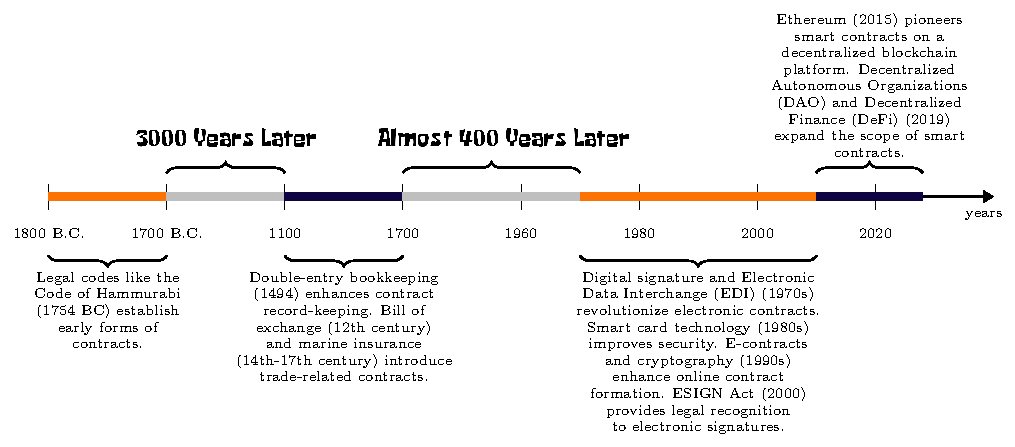
\includegraphics[width=\linewidth]{tikz/chapter4 - Smart Contract Timeline.pdf}
\caption{Smart Contracts Key Inventions Timeline}
\end{figure}


So what is different from a normal contract? In traditional contracts, the verbal text on paper is interpreted by human beings or lawyers ("wet" code). Their legal enforceability is subject to the \textbf{discretionary compliance and semantic flexibility} of human contracts. So, legal validity depends on the willingness of the parties involved to abide by the rules and the ability to interpret the text flexibly and adaptable to the situation.
On the other hand, smart contracts are rules and contracts executed as in a distribution machine ("dry" code). They are legally binding in a technological way, being contracts executed inexorably by code (as \textbf{Lessig} argues: "\textit{code is law}" \cite{les99}), which \textbf{cannot be violated and proceed unstoppably even if conditions have changed}.

\section{Ricardian Contracts}
A Ricardian contract is a legal document that is \textbf{comprehensible and accepted by both humans and machines}, and that is linked to all anticipated future operations (transactions). This type of contract possesses several distinctive properties. First, it is offered by an issuer to holders and represents a right of value managed by the issuer. It is easily readable by people, like a contract on paper, but is also interpretable by programmes, like a database. The contract is digitally signed and contains keys and server information, as well as being associated with a unique and secure identifier. This is basically an \textbf{evolution of the original contract}, indeed each contract can be represented by a graph of objects in prose, interacting in an ecosystem.

\textit{But hey, to really paint the picture, what sets it apart from a smart contract?} Ricardian Contracts focus primarily on being a primary document for the issuance of a digital asset, with an emphasis on \textbf{richer semantics}. In contrast, Smart Contracts are \textbf{more oriented towards programmability} and follow a deterministic approach. So, while Ricardians aim to provide a comprehensive document that is easily understood by all parties involved, Smart Contracts put more emphasis on automating contractual activities through code.

\textit{Let's put it in terms of desserts: Ricardian contracts are like grandma's homemade apple pie - wholesome, comforting, and always a crowd-pleaser. Smart contracts, on the other hand, are more like molecular gastronomy - innovative, impressive, but you're not entirely sure if it's still food...}

\section{Bitcoin or Ethereum? \texorpdfstring{\faBitcoin}{} \ \texorpdfstring{\faEthereum}{}}

Ethereum and Bitcoin differ significantly in their ability to execute smart contracts. \textbf{\textcolor{Orange}{Bitcoin}}, using a full non-Turing script language, is \textbf{limited in its ability to handle complex contracts} or sophisticated decentralised applications. On the other hand, \textbf{\textcolor{Orange}{Ethereum}} offers a \textbf{more powerful environment for smart contracts} through the Solidity language, running on its \textbf{Ethereum virtual machines} (EVMs), which are full Turing. This allows developers to create much more sophisticated smart contracts on Ethereum, with the ability to perform a wide range of calculations or programmable logic. In short, Ethereum offers a more flexible and powerful platform for smart contract development than Bitcoin.

\section{Smart Contract Compliance Issues}
There are several problems with smart contracts that can cause uncertainty and legal challenges:
\begin{enumerate}
    \item \textbf{\textcolor{Blue}{Understanding the Computer Code}}: courts and parties involved may have difficulty understanding the computer code on which smart contracts are based. This can make it difficult to assess all contractual obligations and terms fully and accurately.
    \item \textbf{\textcolor{Blue}{Legal Bindingness}}: in some jurisdictions, the legality and bindingness of smart contracts are not clearly defined. Some courts may not recognise smart contracts as legally binding agreements.
    \item \textbf{\textcolor{Blue}{Determinism of Smart Contracts}}: smart contracts operate deterministically, performing only what they have been programmed to do. This means that they cannot adapt or resolve situations not foreseen in the code.
    \item \textbf{\textcolor{Blue}{Legal Considerations and Exceptions}}: there are many legal considerations and exceptions that must be taken into account when entering into a contract. Smart contracts may not be able to handle these complex situations effectively.
    \item \textbf{\textcolor{Blue}{Different Laws and Jurisdictions}}: laws and jurisdictions vary from country to country. Some jurisdictions may be more favourable to the recognition of smart contracts than others.
\end{enumerate}
Taken together, these factors contribute to smart contracts being subject to legal uncertainty and may require further regulation and clarification to be fully accepted and reliably used.

\textbf{\textcolor{Orange}{Smart Legal Contracts}} are an evolution of traditional smart contracts, offering a solution to address the legal challenges associated with their implementation. While smart contracts consist of computer code and operate according to the "code is law" principle, Smart Legal Contracts combine legal language, parameters and code to create a legally binding contract.

The main objective of Smart Legal Contracts is to provide neutral performance within the terms and conditions defined by the contractual parties. Unlike smart contracts, Smart Legal Contracts recognise that the \textbf{law has the final word and may be subject to legal interpretation and modification}.

In terms of modifiability, Smart Legal Contracts offer \textbf{more flexibility than traditional smart contracts}. While the code of smart contracts cannot be changed once activated, Smart Legal Contracts allow changes to the code and can be paused if necessary.

That's why Smart Legal Contracts find application in a \textbf{wide range of industries and types of agreements}, as they offer a solution for creating legally binding contracts that also incorporate code-based automation and execution elements.

\section{DApps}

Now that we have studied smart contracts in detail, it is time to turn our gaze towards the stars of the show: the DApps. However, before we let ourselves be enchanted by their wonders, it is crucial to take a closer look at the ecosystem that supports them. This overview not only prepares us for the next act, but also shows us the interconnection and synergy between the layers that make the DApp venture possible. 

\begin{figure}[!htbp]
\centering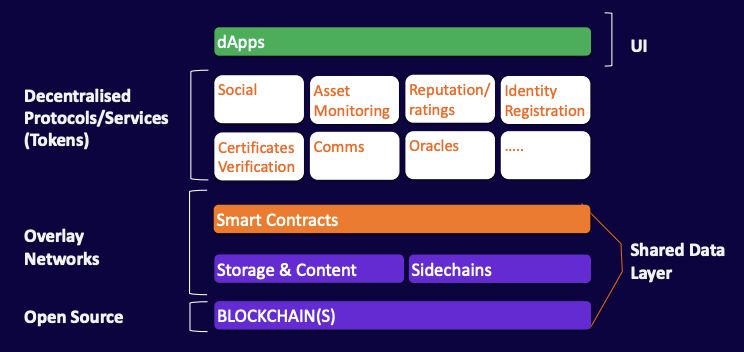
\includegraphics[scale=0.75]{tikz/chapter 4 - Blockchain Stack.png}
\caption{Representation of the Blockchain Stack}
\end{figure}

From bottom to top:
\begin{itemize}
    \item \textbf{Blockchain}: This is the foundation on which the entire ecosystem is based. 
    \item \textbf{Storage, Content and Sidechains}: This layer manages the storage of data and the content associated with transactions on the blockchain. It also includes sidechains, which are separate blockchains connected to the main blockchain. Sidechains allow specific transactions to be performed without clogging up the main blockchain, improving scalability and enabling experimentation with new functionality without compromising security.
    \item \textbf{Smart Contracts}: \textit{We have just seen them :)}
    \item \textbf{Decentralised Protocols and Services}: This layer comprises the decentralised protocols and services that enable the creation, management and exchange of digital tokens on the blockchain. \textbf{Tokens} can represent digital currency, digital assets, rights to use resources and much more. These protocols and services provide a standardised infrastructure to facilitate the interoperability and adoption of tokens within the blockchain ecosystem.
    \item \textbf{DApps}: This is the highest layer of the stack and represents decentralised applications that utilise the layers below to provide a wide range of services and functionality to users. DApps exploit the unique features of blockchain, such as security, immunity from censorship and transparency, to offer innovative and reliable solutions.
\end{itemize}

Basically, decentralised applications are software programmes that operate by different methods. In addition to their underlying architecture and functionality, DApps may also present different \textbf{user interfaces} (UIs) to allow users to interact with them in intuitive and user-friendly ways. They are generally classified into three types: Type 1, Type 2 or Type 3.

\begin{table}[h]
\begin{tabularx}{\linewidth}{>{\parskip1ex}X@{\kern2\tabcolsep}>{\parskip1ex}X@{\kern2\tabcolsep}>{\parskip1ex}X}
\toprule
\hfil\bfseries \color{Orange}{Type 1}
&
\hfil\bfseries \color{Orange}{Type 2}
&
\hfil\bfseries \color{Orange}{Type 3}
\\\cmidrule(r{-\tabcolsep}){1-1}\cmidrule(lr{-\tabcolsep}){2-2}\cmidrule(l{-\tabcolsep}){3-3}

%% TYPE 1
Type 1 DApps operate on their own \textbf{\color{Blue}{dedicated blockchain}}. A prominent example of this is Ethereum-based smart contract DApps. These DApps, such as decentralized finance (DeFi) applications, execute on the Ethereum blockchain and may utilize a native token like ETH.
&
%% TYPE 2
Type 2 DApps utilize an \textbf{\color{Blue}{existing established blockchain}}. They rely on Type 1 blockchains and introduce custom protocols and tokens. For instance, DAI is built on top of Ethereum but features its own stablecoins and mechanisms for distribution and governance.
&
%% TYPE 3
Type 3 DApps leverage the \textbf{\color{Blue}{protocols of Type 2 DApps}}. An example is the SAFE Network, which utilizes the OMNI network protocol. These DApps build upon existing decentralized infrastructure to offer specialized functionalities.
\\
\bottomrule
\end{tabularx}
\caption{Benefits, Limitations, and Additional Considerations of Blockchain Technology}
\end{table}

DApps must be completely open source and autonomous, with no one entity controlling most of their tokens, changes must be based on community consensus, data must be cryptographically secure on a decentralised public blockchain, and a cryptographic token must be used for access and to incentivise contributors, generated by the DApp itself as proof of value.

\section{Oracles}
Unfortunately, smart contracts, and consequently DApps, do not have the ability to directly access external data. However, to overcome this limitation, special tools called \textbf{oracles} come into play. 

In DApps, oracles act as a bridge between the real world and the blockchain, allowing smart contracts to \textbf{access external data} and perform actions in response to certain conditions. Oracles are services provided by third parties and are designed to provide reliable external data to smart contracts on the blockchain. This data can cover a wide range of information, such as weather conditions, payment confirmations or price changes.

The operation of oracles varies depending on the implementation and the blockchain used. In Bitcoin, for example, an oracle can write \textbf{data about a specific transaction}, while in Ethereum, data can be \textbf{stored in the smart contract} itself for use by other smart contracts through message calls.

Oracles are key to enabling DApps to interact with the outside world and perform actions based on real events, thus expanding the possibilities of blockchain usage beyond the confines of the closed system of the blockchain itself.

\section{Blockchain and Smart Contracts Summary}
Here we include schemes that summarise the various concepts we have addressed in these sections:
\begin{figure}[!htbp]
\centering
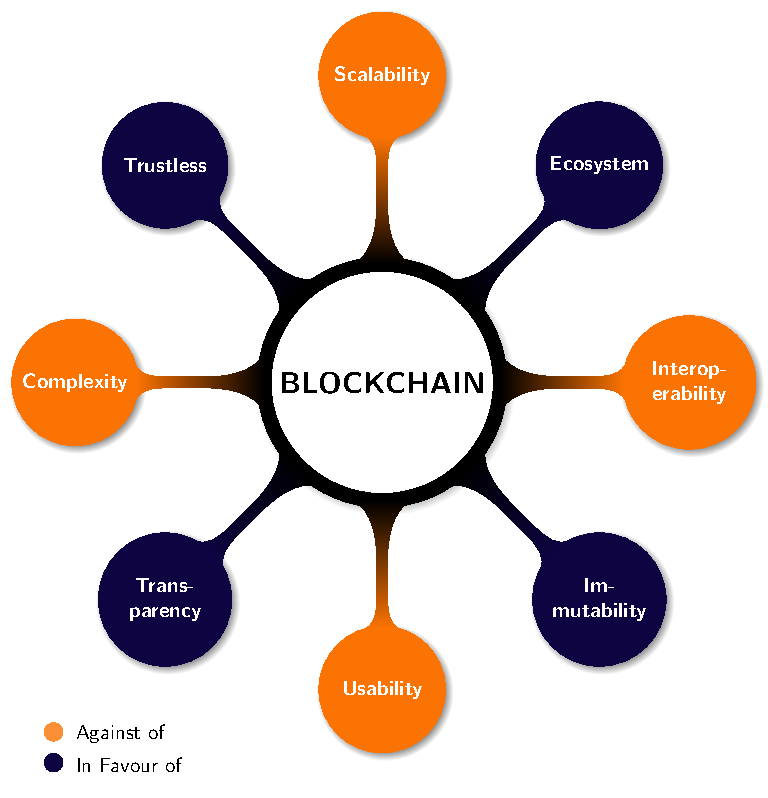
\includegraphics[width=0.7\linewidth]{tikz/chapter4 - Blockchain Summary.pdf}
\caption{Blockchain Concepts Summary}
\end{figure}

\

\begin{figure}[!htbp]
\centering
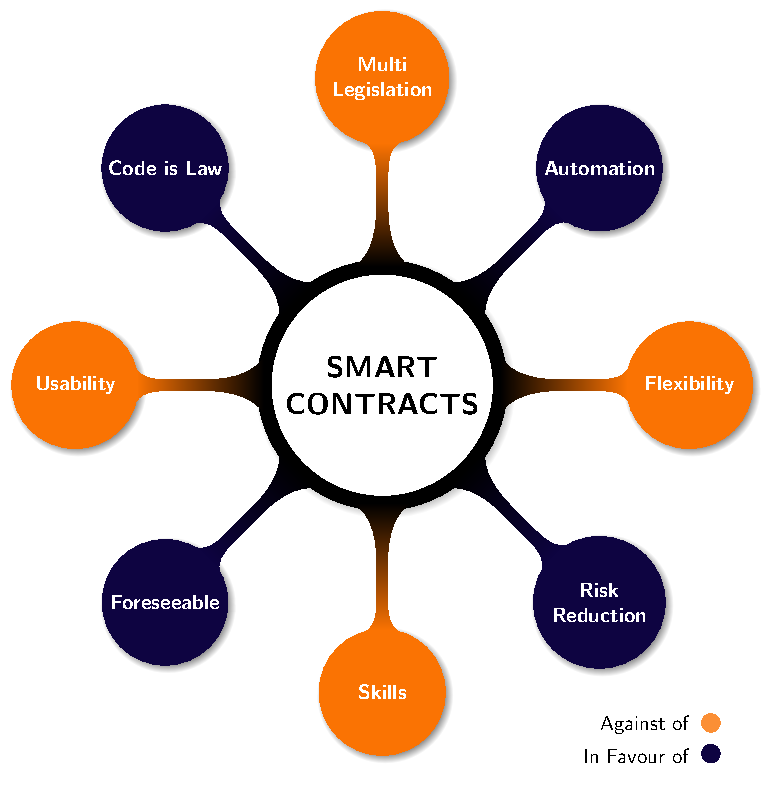
\includegraphics[width=0.7\linewidth]{tikz/chapter4 - Smart Contracts Summary.pdf}
\caption{Smart Contracts Concepts Summary}
\end{figure}

\newpage 
\ % The empty page
\newpage
\listoffigures
\listoftables
%----------------------------------------------------------------------------------------
\newpage
\printbibliography[title = {Bibliography}]

\end{document}
